\documentclass[
  coursetitle={Cómputo Nube y Tecnologías Emergentes},
  coursehours={96},
  coursedate={Verano 2026},
  doctype={Práctica},
  otherlangs={english,french},
  authorname={Lázaro},
  authorsurname={Bustio-Martínez},
  authortitle={PhD},
  role={Profesor Investigador},
  email={lbustio@inaoe.mx},
  phone={5559504000},
  ext={7459},
  institution={Instituto Nacional de Astrofísica, Óptica y Electrónica (INAOE)},
  department={Maestría en Ciencias en Tecnologías de Seguridad},
  address={Luis Enrique Erro 1, Sta. Ma. Tonantzintla, San Andrés Cholula, CP 72840, Puebla, México},
  margin={0.5in}
]{../../lbustio_lecture_notes}

\usepackage[utf8]{inputenc}
\usepackage[T1]{fontenc}
\usepackage{array}
\usepackage{tabularx}
\usepackage{enumitem}
\usepackage{longtable}
\usepackage{booktabs}
\usepackage{url}
\usepackage{listings}
\usepackage{xcolor}
\usepackage{graphicx}
\usepackage{tcolorbox}
\usepackage{amssymb}
\usepackage{tikz}
\usetikzlibrary{arrows.meta,backgrounds,fit,positioning}

\definecolor{lightgray}{rgb}{0.97, 0.97, 0.97}
\definecolor{darkblue}{rgb}{0, 0, 0.6}
\definecolor{cloudblue}{HTML}{1F5FA8}
\definecolor{cloudgreen}{HTML}{2E7D59}
\definecolor{cloudorange}{HTML}{B36B00}
\definecolor{cloudred}{HTML}{A83232}
\definecolor{cloudpurple}{HTML}{5B3F8C}
\definecolor{softgray}{HTML}{F5F7FA}

\newcolumntype{Y}{>{\raggedright\arraybackslash}X}

\lstset{
  backgroundcolor=\color{lightgray},
  basicstyle=\ttfamily\small,
  breaklines=true,
  frame=single,
  columns=fullflexible,
  showstringspaces=false,
  commentstyle=\color{gray},
  keywordstyle=\color{darkblue},
  inputencoding=utf8,
  extendedchars=true,
  literate={á}{{\'a}}1 {é}{{\'e}}1 {í}{{\'i}}1 {ó}{{\'o}}1 {ú}{{\'u}}1 {ñ}{{\~n}}1
}

\setlist[itemize]{topsep=0.3em,itemsep=0.2em}
\setlist[enumerate]{topsep=0.3em,itemsep=0.2em}

\tikzset{
  archbox/.style={
    draw=cloudblue,
    fill=cloudblue!7,
    rounded corners=4pt,
    thick,
    align=center,
    text width=3.6cm,
    minimum height=1.05cm,
    inner sep=6pt,
    font=\small
  },
  archgreen/.style={
    archbox,
    draw=cloudgreen,
    fill=cloudgreen!8
  },
  archorange/.style={
    archbox,
    draw=cloudorange,
    fill=cloudorange!10
  },
  archred/.style={
    archbox,
    draw=cloudred,
    fill=cloudred!7
  },
  archpurple/.style={
    archbox,
    draw=cloudpurple,
    fill=cloudpurple!8
  },
  flowarrow/.style={
    -{Latex[length=3mm,width=2mm]},
    thick,
    draw=darkblue
  },
  returnarrow/.style={
    -{Latex[length=3mm,width=2mm]},
    thick,
    dashed,
    draw=cloudgreen
  }
}

\begin{document}

\IberoCover

\section{Propósito de la sesión}

Esta sesión está destinada a desarrollar, completar y corregir la práctica asignada en la sesión anterior. No se trata de introducir una actividad nueva, sino de usar el tiempo de clase para que cada estudiante avance de forma controlada en la creación de una infraestructura básica en Google Cloud Platform.

Durante la sesión, cada estudiante deberá crear o terminar de configurar una máquina virtual Linux en GCP, conectarse por SSH, instalar software básico, publicar un servidor web mínimo con Nginx, verificar su funcionamiento desde Internet y documentar el proceso en un reporte técnico.

El objetivo central es que el estudiante no entregue solamente capturas aisladas, sino que pueda explicar qué hizo, por qué lo hizo, qué problemas encontró, cómo los resolvió y qué riesgos técnicos o económicos identificó.

\section{Relación con la sesión anterior}

La sesión anterior presentó los elementos básicos de Google Cloud Platform y dejó como práctica la creación de infraestructura básica en la nube. Esta clase práctica retoma esa tarea y la convierte en una sesión de trabajo supervisado.

La actividad se concentra en:

\begin{itemize}
    \item crear o revisar un proyecto en GCP;
    \item crear una máquina virtual Linux en Compute Engine;
    \item seleccionar región, zona, tipo de máquina y disco;
    \item configurar acceso remoto por SSH;
    \item habilitar tráfico HTTP;
    \item instalar Nginx, \texttt{htop} y \texttt{mc};
    \item verificar conectividad local y pública;
    \item documentar evidencias técnicas;
    \item analizar costos, riesgos y problemas encontrados;
    \item detener o eliminar recursos al finalizar.
\end{itemize}

\section{Resultado esperado}

Al terminar la sesión, cada estudiante deberá contar con:

\begin{enumerate}
    \item Una máquina virtual Linux creada en Google Cloud Platform.
    \item Acceso SSH funcional a la máquina virtual.
    \item Nginx instalado y activo.
    \item La página inicial de Nginx visible desde un navegador usando la IP pública de la VM.
    \item \texttt{htop} y \texttt{mc} instalados y ejecutados al menos una vez.
    \item Evidencias suficientes para construir el reporte.
    \item Una bitácora breve de problemas encontrados y soluciones aplicadas.
    \item La VM detenida o eliminada si ya no se utilizará.
\end{enumerate}

\begin{tcolorbox}[title=Producto de la práctica,colback=cloudblue!5,colframe=cloudblue]
La práctica se considera completa cuando el estudiante puede demostrar que desplegó una VM Linux en GCP, accedió por SSH, instaló software, publicó Nginx, verificó acceso desde Internet y documentó el proceso de forma reproducible.
\end{tcolorbox}

\section{Infraestructura requerida}

La infraestructura mínima esperada es la misma de la tarea anterior.

\begin{table}[h]
\centering
\renewcommand{\arraystretch}{1.15}
\begin{tabularx}{\textwidth}{|p{5.2cm}|Y|}
\hline
\textbf{Elemento} & \textbf{Requisito} \\
\hline
Plataforma & Google Cloud Platform \\
\hline
Servicio & Compute Engine \\
\hline
Nombre sugerido de la instancia & \texttt{course} \\
\hline
Sistema operativo & Debian GNU/Linux 12 Bookworm \\
\hline
Arquitectura & \texttt{x86\_64} \\
\hline
Tipo de máquina sugerido & \texttt{e2-small} \\
\hline
CPU & 2 vCPU \\
\hline
Memoria & 1 GB \\
\hline
Disco persistente & 10 GB \\
\hline
Acceso remoto & SSH \\
\hline
Tráfico HTTP & Habilitado \\
\hline
Servidor web & Nginx \\
\hline
Software adicional & \texttt{htop} y \texttt{mc} \\
\hline
\end{tabularx}
\end{table}

\section{Arquitectura de referencia}

\begin{figure}[h]
\centering
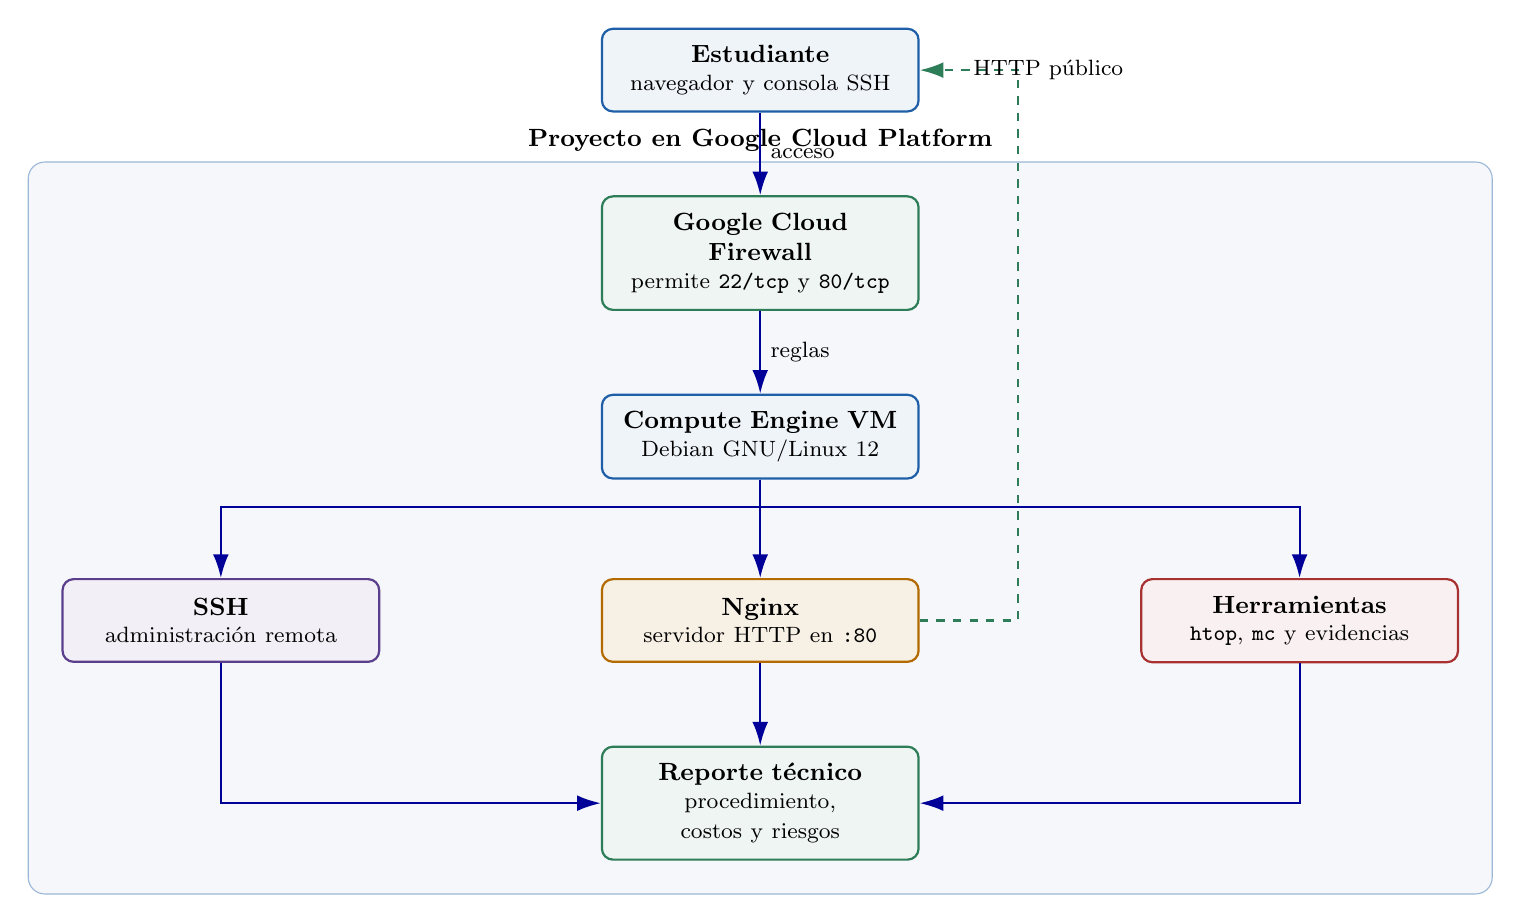
\begin{tikzpicture}[node distance=1.05cm, transform shape]
    \node[archbox] (student) {\textbf{Estudiante}\\[-1pt]\footnotesize navegador y consola SSH};
    \node[archgreen, below=of student] (firewall) {\textbf{Google Cloud Firewall}\\[-1pt]\footnotesize permite \texttt{22/tcp} y \texttt{80/tcp}};
    \node[archbox, below=of firewall] (vm) {\textbf{Compute Engine VM}\\[-1pt]\footnotesize Debian GNU/Linux 12};

    \node[archpurple, below left=1.25cm and 2.8cm of vm] (ssh) {\textbf{SSH}\\[-1pt]\footnotesize administración remota};
    \node[archorange, below=1.25cm of vm] (nginx) {\textbf{Nginx}\\[-1pt]\footnotesize servidor HTTP en \texttt{:80}};
    \node[archred, below right=1.25cm and 2.8cm of vm] (tools) {\textbf{Herramientas}\\[-1pt]\footnotesize \texttt{htop}, \texttt{mc} y evidencias};
    \node[archgreen, below=1.05cm of nginx] (report) {\textbf{Reporte técnico}\\[-1pt]\footnotesize procedimiento, costos y riesgos};

    \draw[flowarrow] (student) -- node[right, font=\footnotesize]{acceso} (firewall);
    \draw[flowarrow] (firewall) -- node[right, font=\footnotesize]{reglas} (vm);
    \draw[flowarrow] (vm.south) -- ++(0,-0.35) -| (ssh.north);
    \draw[flowarrow] (vm.south) -- (nginx.north);
    \draw[flowarrow] (vm.south) -- ++(0,-0.35) -| (tools.north);
    \draw[flowarrow] (ssh.south) |- (report.west);
    \draw[flowarrow] (tools.south) |- (report.east);
    \draw[flowarrow] (nginx) -- (report);
    \draw[returnarrow] (nginx.east) -- ++(1.25,0) |- node[pos=0.78,right,font=\footnotesize]{HTTP público} (student.east);

    \begin{scope}[on background layer]
        \node[
            draw=cloudblue!45,
            fill=softgray,
            rounded corners=6pt,
            inner sep=12pt,
            fit=(firewall) (vm) (ssh) (nginx) (tools) (report),
            label={[font=\small\bfseries]above:Proyecto en Google Cloud Platform}
        ] {};
    \end{scope}
\end{tikzpicture}
\caption{Arquitectura mínima de la práctica: acceso SSH, firewall HTTP y VM Linux con Nginx.}
\end{figure}

\section{Puertos permitidos}

Para esta práctica solo se requieren los puertos mínimos:

\begin{table}[h]
\centering
\renewcommand{\arraystretch}{1.15}
\begin{tabularx}{0.82\textwidth}{|p{2.5cm}|p{3cm}|Y|}
\hline
\textbf{Puerto} & \textbf{Protocolo} & \textbf{Uso} \\
\hline
22 & TCP & Acceso remoto por SSH \\
\hline
80 & TCP & Acceso HTTP al servidor Nginx \\
\hline
\end{tabularx}
\end{table}

No se deben abrir puertos adicionales salvo indicación explícita del profesor.

\section{Organización de la clase}

\subsection{Revisión inicial}

Cada estudiante debe verificar si ya cuenta con:

\begin{itemize}
    \item acceso a su cuenta de GCP;
    \item proyecto creado o seleccionado;
    \item facturación habilitada si GCP lo solicita;
    \item acceso a Compute Engine;
    \item VM creada o lista para crearse;
    \item notas de avance de la tarea anterior.
\end{itemize}

Si algún estudiante no pudo iniciar la tarea, debe comenzar desde la creación del proyecto y la VM.

\subsection{Creación o revisión de la VM}

Los estudiantes que ya tengan la VM creada deberán revisar:

\begin{itemize}
    \item nombre de la instancia;
    \item sistema operativo;
    \item región y zona;
    \item tipo de máquina;
    \item disco persistente;
    \item IP pública;
    \item reglas de firewall;
    \item estado de la instancia.
\end{itemize}

Los estudiantes que aún no tengan la VM deberán crearla siguiendo los requisitos de la tarea.

\subsection{Conexión SSH}

Cada estudiante debe conectarse a la VM mediante SSH desde la consola de GCP.

Al entrar a la máquina, se recomienda ejecutar:

\begin{lstlisting}
hostname
whoami
uname -a
cat /etc/os-release
free -h
df -h
\end{lstlisting}

Estas salidas sirven como evidencia de acceso, sistema operativo, memoria y disco.

\subsection{Instalación de software}

Dentro de la VM, se deben instalar los paquetes obligatorios:

\begin{lstlisting}
sudo apt update
sudo apt install -y nginx htop mc
\end{lstlisting}

Después de la instalación, se debe verificar el estado de Nginx:

\begin{lstlisting}
systemctl status nginx
\end{lstlisting}

También se puede usar:

\begin{lstlisting}
sudo systemctl is-active nginx
\end{lstlisting}

El resultado esperado es que el servicio aparezca como activo.

\subsection{Verificación local de Nginx}

Desde la propia VM:

\begin{lstlisting}
curl http://localhost
\end{lstlisting}

Si Nginx está funcionando, la terminal debe mostrar el contenido HTML de la página inicial.

\subsection{Verificación desde navegador externo}

Cada estudiante debe copiar la IP pública de su VM y abrirla en un navegador:

\begin{lstlisting}
http://DIRECCION_IP_PUBLICA
\end{lstlisting}

La evidencia debe mostrar la página inicial de Nginx cargando desde Internet.

Si la página no responde, se deben revisar:

\begin{itemize}
    \item estado de la VM;
    \item IP pública correcta;
    \item regla de firewall para HTTP;
    \item casilla de permitir tráfico HTTP;
    \item estado del servicio Nginx;
    \item errores de red del navegador.
\end{itemize}

\subsection{Verificación de herramientas adicionales}

Ejecutar:

\begin{lstlisting}
htop
\end{lstlisting}

Tomar evidencia de la interfaz de monitoreo. Para salir, usar \texttt{F10} o \texttt{q}.

Ejecutar:

\begin{lstlisting}
mc
\end{lstlisting}

Tomar evidencia del administrador de archivos en terminal. Para salir, usar \texttt{F10}.

\section{Guía de troubleshooting}

Durante la clase se espera que aparezcan errores. El objetivo no es evitarlos, sino aprender a diagnosticarlos.

\subsection{No puedo conectarme por SSH}

Revisar:

\begin{itemize}
    \item que la VM esté encendida;
    \item que la cuenta de GCP tenga permisos suficientes;
    \item que no haya errores temporales en la consola;
    \item que el navegador permita ventanas emergentes si se usa SSH desde GCP;
    \item que la regla de firewall para SSH no haya sido modificada de forma incorrecta.
\end{itemize}

\subsection{Nginx no instala}

Probar:

\begin{lstlisting}
sudo apt update
sudo apt install -y nginx
\end{lstlisting}

Si hay errores, documentar:

\begin{itemize}
    \item mensaje exacto;
    \item comando ejecutado;
    \item solución intentada;
    \item resultado final.
\end{itemize}

\subsection{Nginx instala pero no responde}

Revisar:

\begin{lstlisting}
sudo systemctl status nginx
sudo systemctl restart nginx
curl http://localhost
\end{lstlisting}

Si responde localmente pero no desde navegador, el problema probablemente está en firewall, IP pública o regla HTTP.

\subsection{La página no abre desde Internet}

Revisar en GCP:

\begin{itemize}
    \item que la VM tenga IP pública;
    \item que la URL use \texttt{http://} y no \texttt{https://};
    \item que el puerto 80 esté permitido;
    \item que la regla de firewall aplique a la instancia correcta;
    \item que Nginx esté activo.
\end{itemize}

\subsection{Aparecen costos inesperados}

Revisar:

\begin{itemize}
    \item tipo de máquina seleccionado;
    \item región;
    \item disco;
    \item recursos activos;
    \item advertencias del estimador de costos;
    \item si la VM quedó encendida después de la práctica.
\end{itemize}

Al finalizar, detener o eliminar la VM si ya no se utilizará.

\section{Evidencias mínimas para reunir durante la clase}

El reporte debe incluir evidencias claras de:

\begin{enumerate}
    \item Proyecto utilizado en GCP.
    \item Instancia \texttt{course} creada en Compute Engine.
    \item Configuración general de la VM.
    \item Sistema operativo Debian GNU/Linux 12.
    \item Región y zona seleccionadas.
    \item Tipo de máquina y disco.
    \item IP pública asignada.
    \item Tráfico HTTP habilitado.
    \item Conexión SSH exitosa.
    \item Comandos de instalación ejecutados.
    \item Estado activo de Nginx.
    \item Prueba con \texttt{curl http://localhost}.
    \item Página de Nginx visible desde navegador externo.
    \item Ejecución de \texttt{htop}.
    \item Ejecución de \texttt{mc}.
    \item Problemas encontrados y soluciones aplicadas.
    \item Costo observado o estimado.
    \item Evidencia de VM detenida o eliminada al finalizar.
\end{enumerate}

\section{Bitácora técnica de la sesión}

Cada estudiante debe mantener una bitácora breve mientras trabaja. Puede usar la siguiente estructura:

\begin{table}[h]
\centering
\renewcommand{\arraystretch}{1.35}
\begin{tabularx}{\textwidth}{|p{1.55cm}|Y|Y|Y|Y|}
\hline
\textbf{Hora} & \textbf{Acción realizada} & \textbf{Resultado} & \textbf{Problema encontrado} & \textbf{Solución aplicada} \\
\hline
 & & & & \\
\hline
 & & & & \\
\hline
 & & & & \\
\hline
\end{tabularx}
\end{table}

Esta bitácora no sustituye al reporte, pero ayuda a construirlo con evidencia real.

\section{Estructura sugerida del reporte}

El entregable debe ser un PDF con la siguiente estructura:

\begin{enumerate}
    \item Portada.
    \item Introducción.
    \item Objetivo de la práctica.
    \item Descripción del proyecto en GCP.
    \item Descripción de la VM creada.
    \item Configuración de red, SSH y firewall.
    \item Instalación de Nginx, \texttt{htop} y \texttt{mc}.
    \item Verificación del servidor web.
    \item Evidencias de funcionamiento.
    \item Problemas encontrados y soluciones aplicadas.
    \item Costos observados o estimados.
    \item Riesgos identificados.
    \item Conclusiones.
\end{enumerate}

\section{Preguntas de análisis para el reporte}

El reporte debe responder de forma breve:

\begin{enumerate}
    \item ¿Qué función cumple Compute Engine dentro del modelo IaaS?
    \item ¿Qué elementos fueron necesarios para que la VM quedara funcional?
    \item ¿Por qué se necesita SSH en esta práctica?
    \item ¿Qué implica exponer el puerto 80 a Internet?
    \item ¿Qué evidencia demuestra que Nginx quedó funcionando?
    \item ¿Qué utilidad tienen \texttt{htop} y \texttt{mc} en una VM Linux?
    \item ¿Qué riesgos existen al dejar una VM encendida sin supervisión?
    \item ¿Qué problemas técnicos aparecieron y cómo se resolvieron?
    \item ¿Qué decisiones podrían reducir costos o riesgos?
\end{enumerate}

\section{Criterios de revisión durante la clase}

El profesor revisará avances con base en:

\begin{table}[h]
\centering
\renewcommand{\arraystretch}{1.15}
\begin{tabularx}{\textwidth}{|p{5.1cm}|Y|}
\hline
\textbf{Criterio} & \textbf{Evidencia esperada} \\
\hline
VM creada correctamente & Instancia visible en Compute Engine \\
\hline
Acceso SSH funcional & Terminal conectada a la VM \\
\hline
Configuración de red adecuada & IP pública y HTTP habilitado \\
\hline
Nginx funcionando & Servicio activo y página visible \\
\hline
Herramientas instaladas & Evidencia de \texttt{htop} y \texttt{mc} \\
\hline
Documentación técnica & Capturas, comandos y bitácora \\
\hline
Análisis crítico & Riesgos, costos y problemas explicados \\
\hline
\end{tabularx}
\end{table}

\section{Reglas de seguridad y buenas prácticas}

\begin{tcolorbox}[title=Seguridad mínima,colback=cloudred!5,colframe=cloudred]
\begin{itemize}
    \item No publicar contraseñas, llaves privadas, tokens ni credenciales.
    \item No abrir puertos que no sean necesarios.
    \item No usar tipos de máquina costosos.
    \item No dejar recursos encendidos sin necesidad.
    \item No copiar reportes genéricos de Internet.
    \item No presentar capturas que no correspondan a la práctica realizada.
    \item Detener o eliminar la VM al finalizar si no se seguirá usando.
\end{itemize}
\end{tcolorbox}

\section{Entregable de la sesión}

Cada estudiante deberá entregar un reporte técnico en PDF sobre lo realizado durante la práctica.

Nombre sugerido del archivo:

\begin{lstlisting}
Tarea2_ApellidoNombre.pdf
\end{lstlisting}

El reporte debe contener procedimiento, evidencias, problemas encontrados, soluciones, costos, riesgos y reflexión final.

\section{Cierre de la sesión}

Antes de salir de clase, cada estudiante debe verificar:

\begin{itemize}
    \item que tiene evidencias suficientes para el reporte;
    \item que documentó los comandos principales;
    \item que anotó problemas y soluciones;
    \item que revisó costos;
    \item que la VM fue detenida o eliminada si ya no se utilizará.
\end{itemize}

\end{document}
